\documentclass[%
 reprint,
%superscriptaddress,
%groupedaddress,
%unsortedaddress,
%runinaddress,
%frontmatterverbose, 
%preprint,
%showpacs,preprintnumbers,
%nofootinbib,
%nobibnotes,
%bibnotes,
 amsmath,amssymb,
 aps,
%pra,
%prb,
%rmp,
%prstab,
%prstper,
%floatfix,
]{revtex4-1}

\usepackage{graphicx}% Include figure files
\usepackage{dcolumn}% Align table columns on decimal point
\usepackage{bm}% bold math
%\usepackage{hyperref}% add hypertext capabilities
%\usepackage[mathlines]{lineno}% Enable numbering of text and display math
%\linenumbers\relax % Commence numbering lines

%\usepackage[showframe,%Uncomment any one of the following lines to test 
%%scale=0.7, marginratio={1:1, 2:3}, ignoreall,% default settings
%%text={7in,10in},centering,
%%margin=1.5in,
%%total={6.5in,8.75in}, top=1.2in, left=0.9in, includefoot,
%%height=10in,a5paper,hmargin={3cm,0.8in},
%]{geometry}

\usepackage{cmap} % Поиск в PDF
\usepackage[T2A]{fontenc} % Кодировка
\usepackage[utf8]{inputenc} % Кодировка исходного текста
\usepackage[english, russian]{babel} % Локализация и переносы
\frenchspacing % Более тонкая настройка пробелов 
\usepackage{multirow}
\usepackage[warn]{mathtext}
\usepackage{amssymb}
\usepackage{ dsfont }
\usepackage{ textcomp }
\usepackage{ mathrsfs }

% Переопределение англоязычного начертания каппа, фи и эпсилон, 
% а также знаков сравнения
\renewcommand{\epsilon}{\ensuremath{\varepsilon}}
\renewcommand{\phi}{\ensuremath{\varphi}} 
\renewcommand{\kappa}{\ensuremath{\varkappa}}
\renewcommand{\le}{\ensuremath{\leslant}}
\renewcommand{\leq}{\ensuremath{\leqslant}}
\renewcommand{\ge}{\ensuremath{\geslant}}
\renewcommand{\geq}{\ensuremath{\geqslant}}
\renewcommand{\emptyset}{\ensuremath{\varnothing}}

\usepackage{textcomp} 
\usepackage{indentfirst} % Красная строка
\usepackage{amsmath} % Текст в формулах
\usepackage{graphicx} % Графика
\DeclareGraphicsExtensions{.pdf,.png,.jpg}
\usepackage{pgfplots}
\pgfplotsset{compat=1.13}

%\usepackage{times}

\begin{document}

\title{Дифракция света на ультразвуковой волне в жидкости}
\thanks{4.3.2}

\author{Иван Едигарьев}
\affiliation{
 Московский Физико-Технический Институт\\
 Факультет Общей и Прикладной Физики, 526т\\
}
%\date{\today}

\begin{abstract}
Цель работы: изучение дифракции света на синусоидальной акустической решётке и наблюдение фазовой решетки методом тёмного поля.
В работе используются: оптическая скамья, осветитель, два длиннофокусных объектива, кювета с жидкостью, кварцевый излучатель с микрометрическим винтом, генератор ультразвуковой частоты, линза, вертикальная нить на рейтере, микроскоп.

\end{abstract}

\pacs{Valid PACS appear here}

\maketitle

\begin{enumerate}

    \item 
    
    \textbf{Определение скорости ультразвука по дифракционной картине.}\\
    
    а) Соберём схему. Включим осветитель. Максимально откроем входную щель.

    б) Поместив лист бумаги между коллиматором и кюветой, убедимся, что световое пятно равномерно освещено; затем проверим освещённость пятна на выходе из прибора.
    
    в) Настроим микроскоп и отсчётное устройство. Установим рабочую ширину щели 20–30 мкм.
    
    Получим дифракционную картину. Картина видна наиболее чётко, когда в кювете образуется стоячая УЗ-волна. 
    
    Определим положения дифракционных полос. Повторим измерения для трёх–четырёх фиксированных частот, лежащих в одном из диапазонов. 
    
    Построим на одном листе графики $Y = Y(m)$ (от $−m$ до $+m$). 
    \begin{figure}[h]
    \center{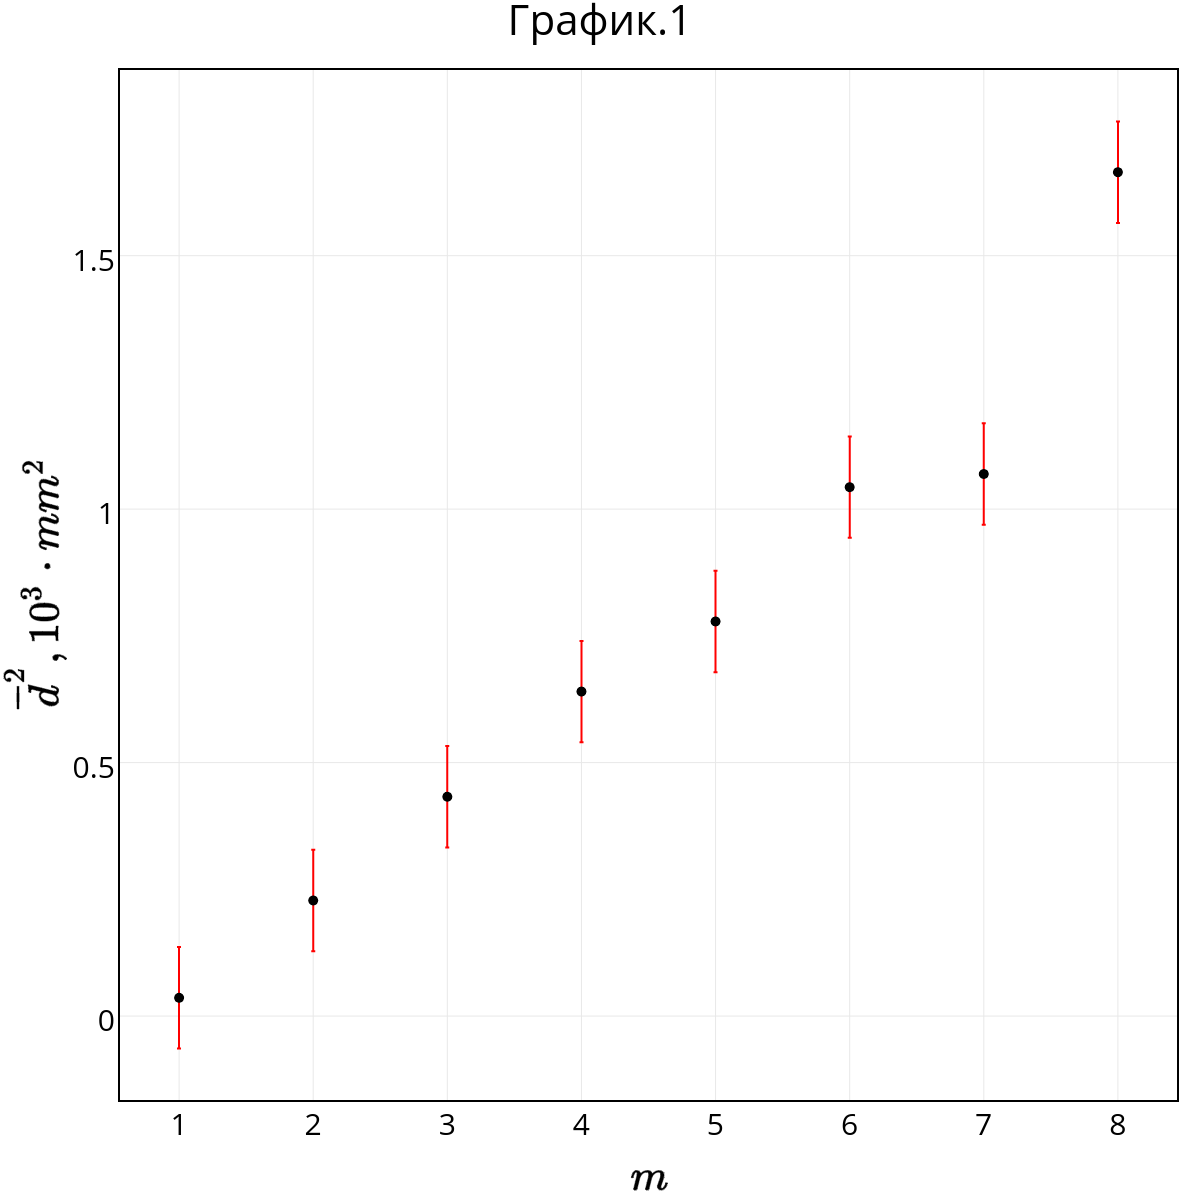
\includegraphics[scale=0.17]{my_plot1.png}}
    \end{figure}
    
    Для каждой частоты определим по наклону прямой расстояние между соседними полосами (цена деления микрометрического винта - 4 мкм). 
    \begin{gather*}
        b_{\nu_1} = (118 \pm 4)~10^{-6}~m,\\
        b_{\nu_2} = (107 \pm 4)~10^{-6}~m,\\
        b_{\nu_3} = (122 \pm 4)~10^{-6}~m.
    \end{gather*}
    
    Зная фокусное расстояние объектива ($f$ = 28 см) и полосу пропускания красного фильтра ($\lambda = 6400 \pm 200$ \AA), рассчитаем длину УЗ-волны $\Lambda$.
    \begin{gather*}
        \Lambda_{\nu_1} = (14 \pm 2)~10^{-4}~m,\\
        \Lambda_{\nu_2} = (17 \pm 3)~10^{-4}~m,\\
        \Lambda_{\nu_3} = (15 \pm 2)~10^{-4}~m.
    \end{gather*}
    
    Рассчитаем скорость звука для каждой частоты и среднюю скорость.
    \begin{gather*}
        v_{\nu_1} = (1600 \pm 100)~m / s,\\
        v_{\nu_2} = (1900 \pm 200)~m / s,\\
        v_{\nu_3} = (1800 \pm 200)~m / s.
    \end{gather*}
    
    \begin{gather*}
        v_{mean} = (1800 \pm 200)~m / s,\\
    \end{gather*}
    
    
    \item 

    \textbf{Определение скорости ультразвука методом тёмного поля.}\\
    
    Настроим установку на метод тёмного поля.
    
    Закроем нулевой дифракционный максимум проволочкой. Меняя частоту, пронаблюдаем акустическую решётку. Убедимся, что при удалении проволочки с главного максимума решётка не видна.
    
    Зафиксируем с помощью окулярной шкалы микроскопа координаты первой и последней из хорошо видимых в поле зрения тёмных полос и количество светлых промежутков между ними.
    
    Повторим измерения для нескольких частот внутри одной из рабочих полос УЗ-излучателя.
    
    \begin{figure}[h]
    \center{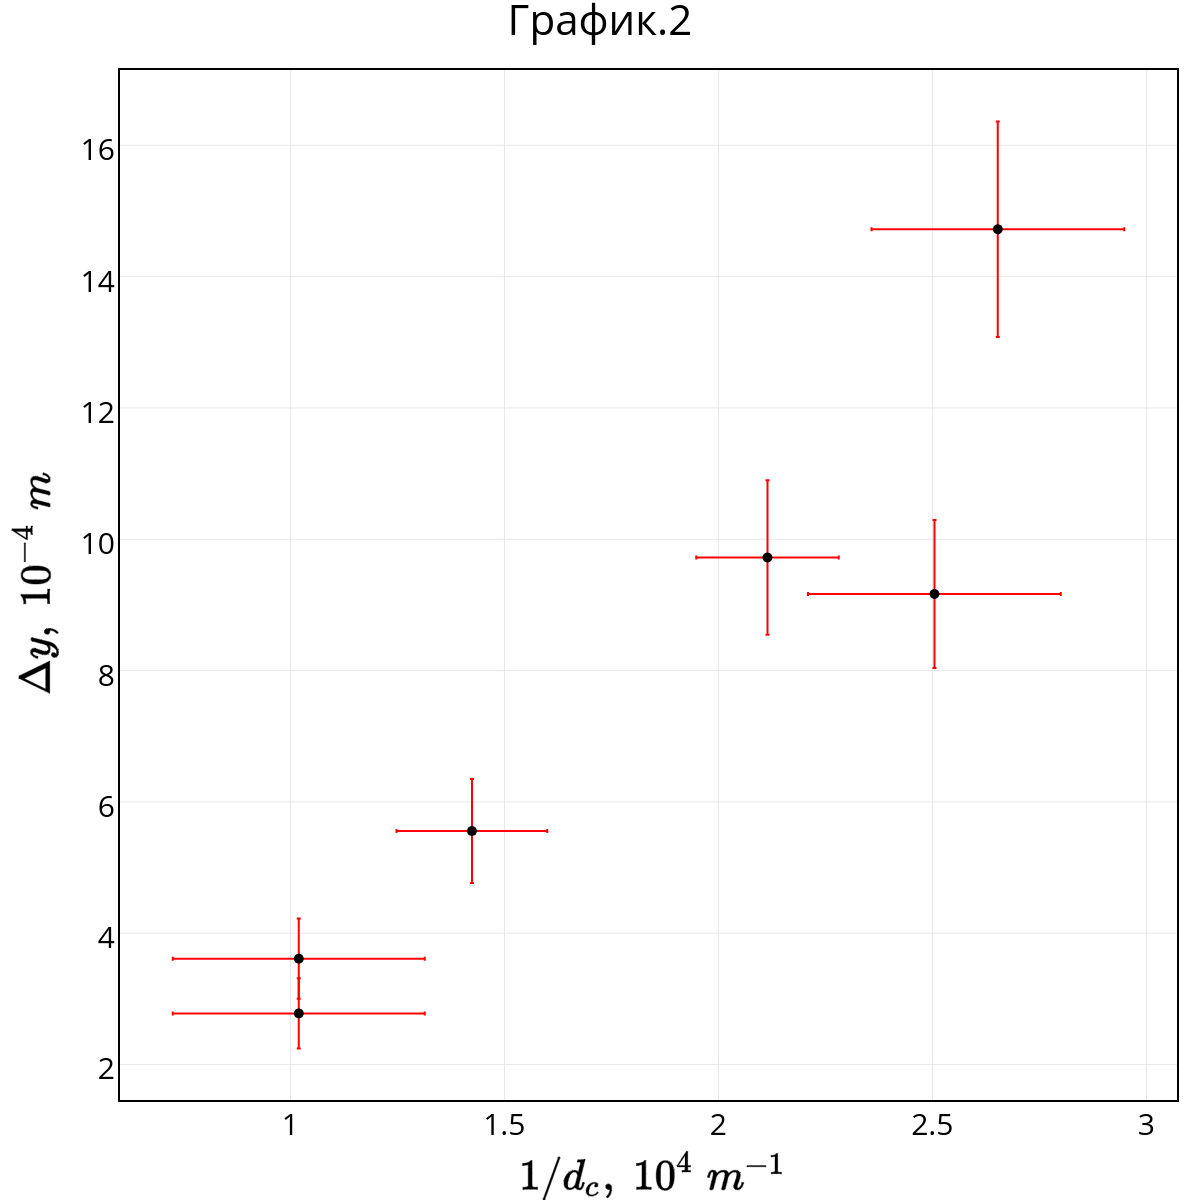
\includegraphics[scale=0.17]{my_plot2.png}}
    \end{figure}
    
    Для каждой частоты рассчитаем длину УЗ-волны $\Lambda$ с учётом удвоения числа наблюдаемых полос.
    
    Построим график $\Lambda = F(1/\nu)$ и определим по наклону прямой скорость ультразвука в воде.
    \begin{gather*}
        b = v = (2600 \pm 200)~m / s.
    \end{gather*}
    
    Табличное значение скорости звука в воде при температуре $20^{\circ}С$:
    \begin{gather*}
        v_{\text{табл}} = 1481~m / s.
    \end{gather*}

\end{enumerate}

\end{document}
